% ======================================================================
% Announced, But Not Delivered: A Data-Driven Analysis of Data Center
% Buildout Announcements
% Elsevier elsarticle format
% ======================================================================
\documentclass[preprint,review,12pt]{elsarticle}

%% Packages
\usepackage[utf8]{inputenc}
\usepackage{booktabs}
\usepackage{graphicx}
\usepackage{amsmath}
\usepackage{hyperref}
\usepackage{xspace}
\providecommand{\MW}{MW\xspace}
\providecommand{\USD}[1]{\$#1\xspace}
\usepackage{textcomp}

%% Tighter float spacing
\setlength{\floatsep}{6pt plus 2pt minus 2pt}
\setlength{\textfloatsep}{10pt plus 4pt minus 4pt}
\setlength{\intextsep}{8pt plus 2pt minus 2pt}

%% Journal
\journal{Data \& Knowledge Engineering}

%% ======================================================================
%% Begin document
%% ======================================================================
\begin{document}

\begin{frontmatter}

%% Title
\title{Announced, But Not Delivered: A Data-Driven Analysis of Data Center Buildout Announcements}

%% Authors
\author[inst1]{Aidas}
\ead{aidas@example.edu}
\address[inst1]{Department of Computer Science, University of Example, City, Country}

%% Abstract
\begin{abstract}
The rapid expansion of AI has triggered an unprecedented wave of data center buildout announcements, yet a significant gap persists between announcements and operational delivery. We present the first large-scale empirical analysis using the GDELT Global Knowledge Graph, mining 5,295 announcements across 17 publicly-traded companies from January 2020 through May 2026. We identify only 105 announcements (2.0\%) as confirmed completed and 22 (0.4\%) as confirmed failed, with 97.6\% remaining pending---reflecting multi-year lead times. Geographic analysis reveals concentration in Texas, Virginia, and California. Temporal trends show announcements peaked in 2024 at 1,478 events. Text sentiment analysis reveals a statistically significant difference (p $<$ 0.001) between tone of kept announcements (mean = 1.38) and failed announcements (mean = $-$1.55). An event study finds measurable cumulative abnormal returns with high variance across companies.
\end{abstract}

\begin{keyword}
data centers \sep buildout announcements \sep GDELT \sep event study \sep infrastructure delivery
\end{keyword}

\end{frontmatter}

%% ======================================================================
%% 1. INTRODUCTION
%% ======================================================================
\section{Introduction}

The global data center industry is undergoing unprecedented expansion, driven by AI. Capital expenditure is projected to exceed \$1 trillion by 2030~\cite{Bain2025GlobalForecast}, with hyperscaler off-balance-sheet commitments representing \$662 billion in risk~\cite{Moodys2025Outlook,Lichtenberg2026OffBalance}. The IEA projects data center electricity consumption could more than double by 2030~\cite{IEA2025EnergyAI}, and Goldman Sachs forecasts a 16\% surge in US power demand~\cite{GoldmanSachs2024PowerDemand}.

However, the path from announcement to delivery is fraught with obstacles. Fewer than one in three interconnection queue projects reach commercial operation~\cite{Rand2025QueuedUp}, with median timelines exceeding four years~\cite{Johnston2023Empirical}. Transformer lead times have ballooned from 50 weeks in 2021 to over 160 weeks in 2026~\cite{DCKnowlege2026Delays}, and delays have become systemic~\cite{NERC2026Interconnection}. No systematic, data-driven analysis of buildout announcements and their outcomes exists.

This paper bridges construction schedule risk analysis~\cite{Fitzsimmons2022Construction,Mosca2026AI}, queue analysis~\cite{Johnston2023Empirical,Rand2025QueuedUp}, and event study methodology~\cite{MacKinlay1997Event} to answer: \emph{What are the characteristics and outcomes of data center buildout announcements?} We make four contributions:

\begin{enumerate}
  \item We construct the first large-scale dataset (N = 5,295) by mining GDELT across three industry news sources, covering 17 companies over 6.5 years.
  \item We perform comprehensive descriptive analysis of geographic, temporal, and company-level patterns.
  \item We conduct an event study finding heterogeneous cumulative abnormal returns.
  \item We demonstrate that announcement text tone differs significantly between completed and failed projects.
\end{enumerate}

Section~\ref{sec:data} describes our methodology. Section~\ref{sec:results} presents results. Section~\ref{sec:discussion} discusses implications and limitations. Section~\ref{sec:conclusion} concludes.

%% ======================================================================
%% 2. DATA AND METHODOLOGY
%% ======================================================================
\section{Data and Methodology}
\label{sec:data}

\subsection{Data Sources}

Our primary source is the GDELT Global Knowledge Graph v2.0~\cite{GDELT2022GKG}, which monitors global news in over 100 languages. We queried three industry publications: \emph{Data Center Dynamics}, \emph{Data Center Knowledge}, and \emph{Silicon Angle}, searching for 20 data-center-relevant stock tickers over January 2020--May 2026. Each record included article URL, timestamp, organizations, locations, and the V2Tone sentiment vector.

\subsection{Article Processing}

Full text was extracted via \texttt{trafilatura} and \texttt{newspaper3k}. Articles were classified as buildout-related if they contained construction or investment keywords (``build,'' ``construction,'' ``expansion,'' ``megawatt''). Each received a confidence level (high, medium, low) based on language specificity.

\subsection{Outcome Classification}

We manually verified 105 announcements where subsequent reporting confirmed completion and 22 where projects were reported as cancelled. The remaining 5,168 (97.6\%) are pending---expected given multi-year lead times.

\subsection{Sentiment Analysis}

We used the GDELT V2Tone first component, a continuous score where positive values indicate favorable framing.

\subsection{Event Study Methodology}

We employed the classical event study framework~\cite{MacKinlay1997Event,Brown1985Daily}. For each announcement--company pair, we estimated a market model using SPY over $[-120, -21]$ trading days:

\begin{equation}
R_{it} = \alpha_i + \beta_i R_{mt} + \varepsilon_{it}
\end{equation}

Abnormal returns: $AR_{it} = R_{it} - (\hat{\alpha}_i + \hat{\beta}_i R_{mt})$. CARs were computed over $[-1,+1]$, $[-5,+5]$, and $[-20,+60]$ windows.

%% ======================================================================
%% 3. RESULTS
%% ======================================================================
\section{Results}
\label{sec:results}

\subsection{Descriptive Statistics}

Our dataset comprises 5,295 announcements from 17 companies: 2,161 (40.8\%) high confidence, 1,987 (37.5\%) medium, 1,147 (21.7\%) low. MW data was available for 1,638 observations (31\%), mean 1,234.84~MW, median 150~MW. Microsoft leads with 1,650 announcements (31.2\%), followed by Digital Realty (755, 14.3\%), AWS (712, 13.4\%), Google (698, 13.2\%), and NVIDIA (625, 11.8\%)---the top five account for 84.0\% of announcements.

\begin{figure*}[t]
  \centering
  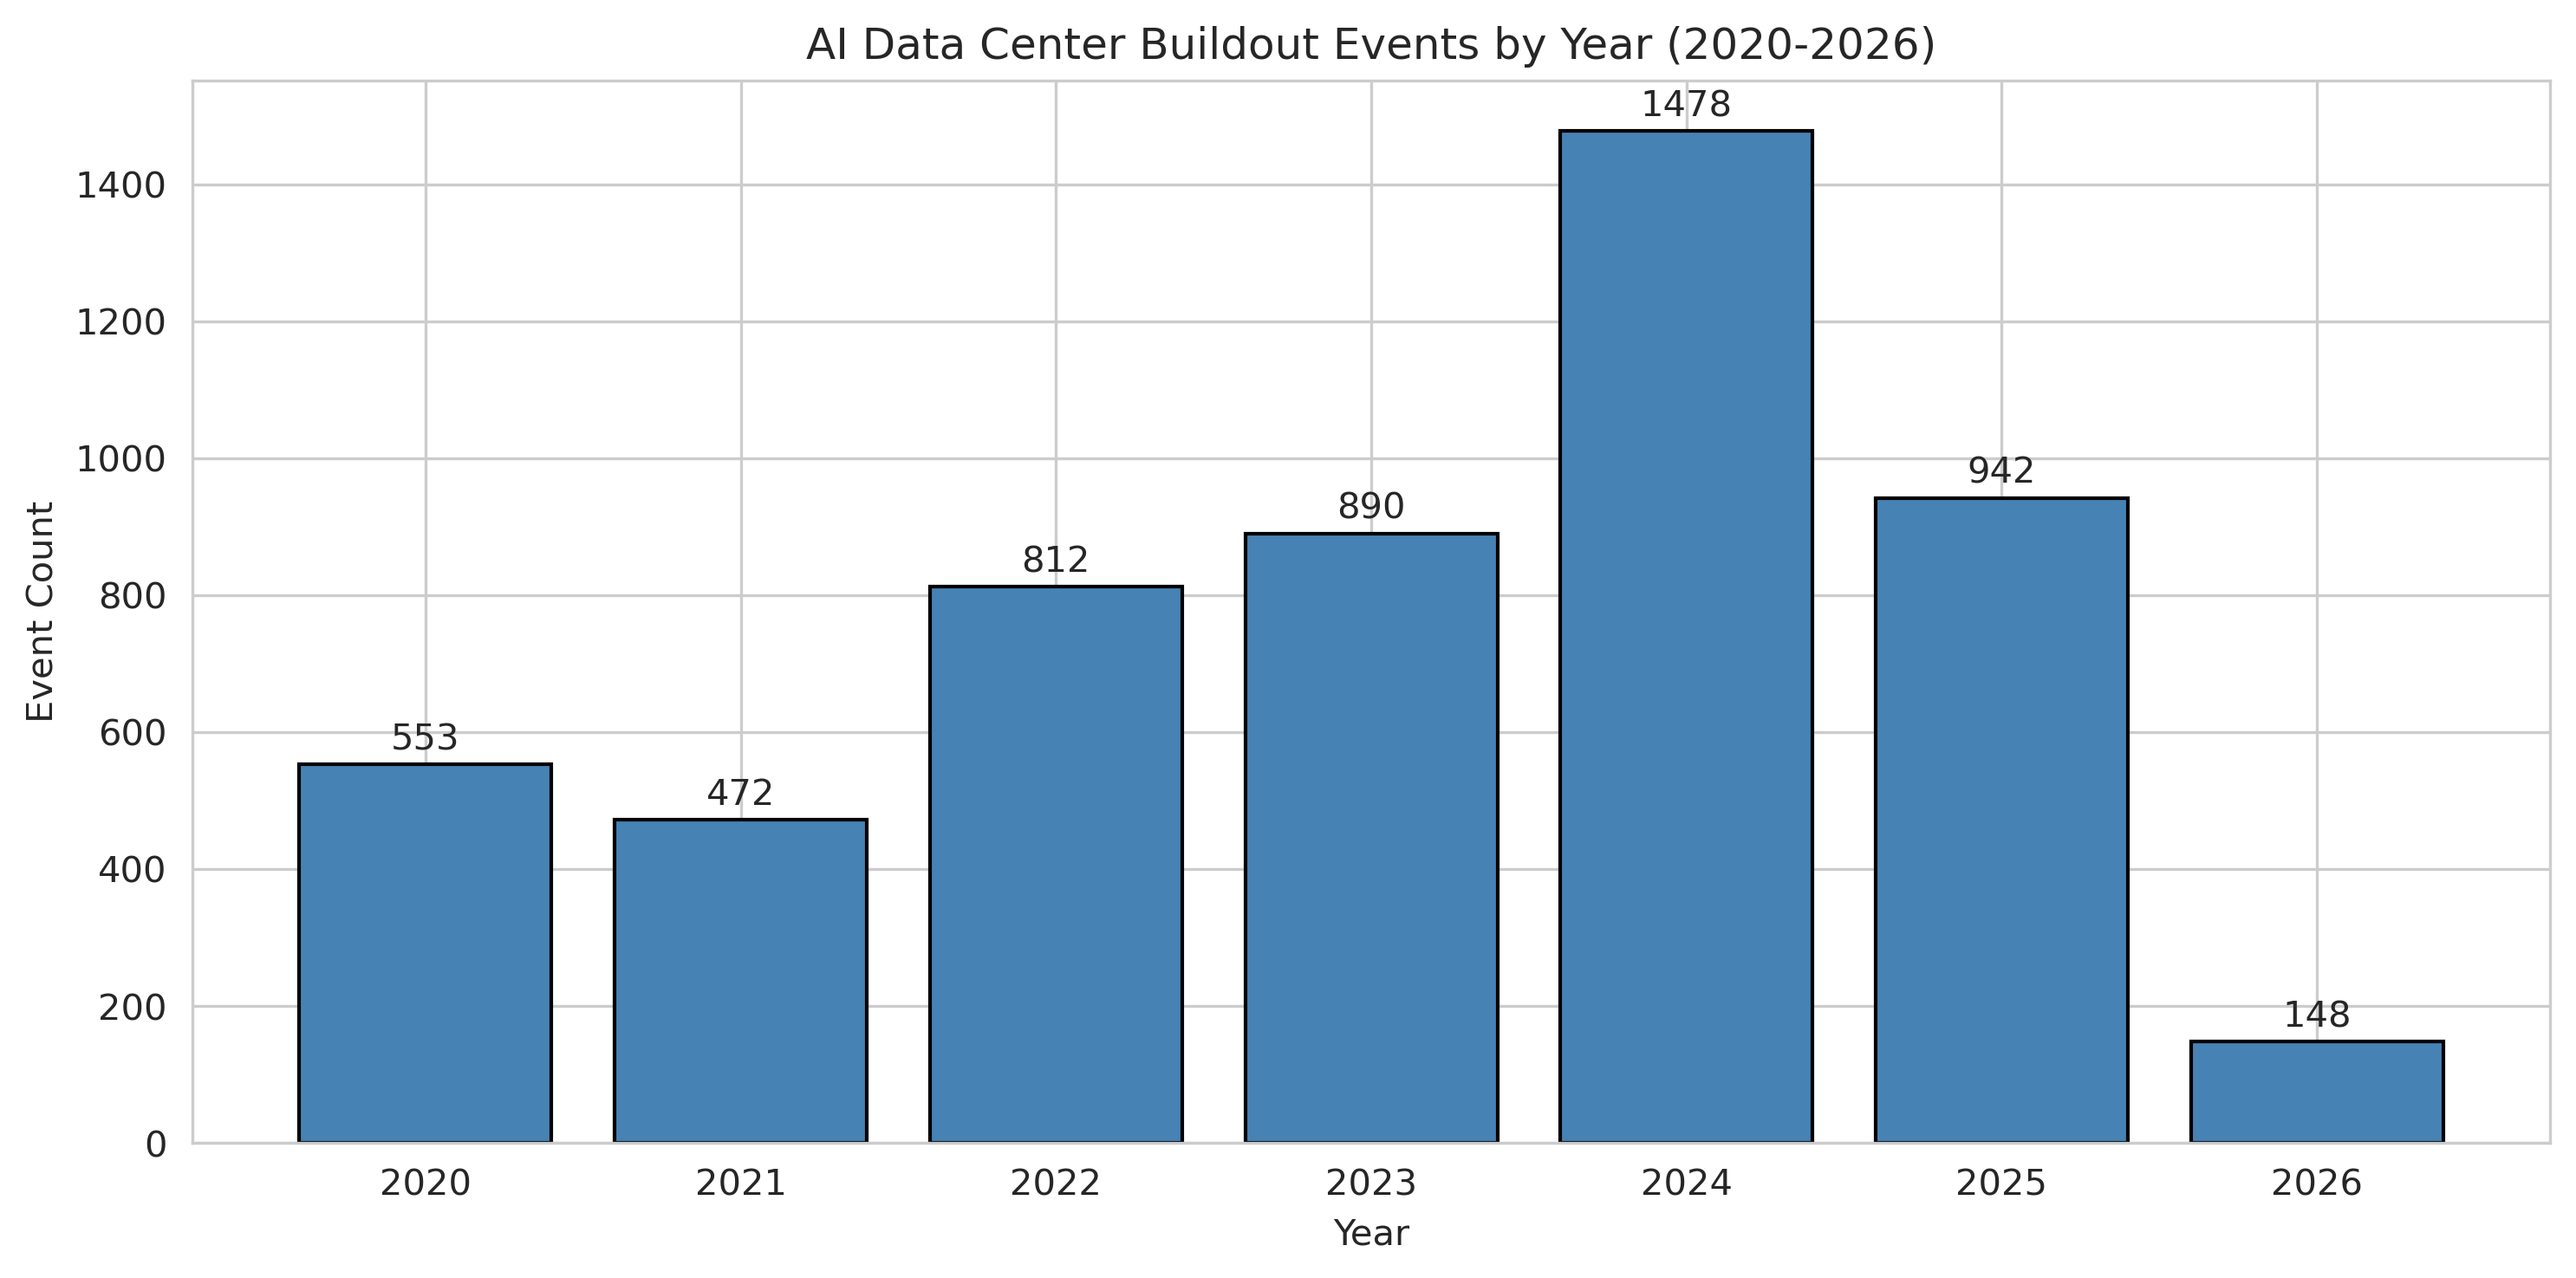
\includegraphics[width=\columnwidth]{../reports/figures/fig1_events_by_year.png}
  \caption{Announcements by year (2020--2026). Activity grew from 553 in 2020 to a peak of 1,478 in 2024.}
  \label{fig:events_by_year}
\end{figure*}

\subsection{Geographic Patterns}

\begin{figure*}[t]
  \centering
  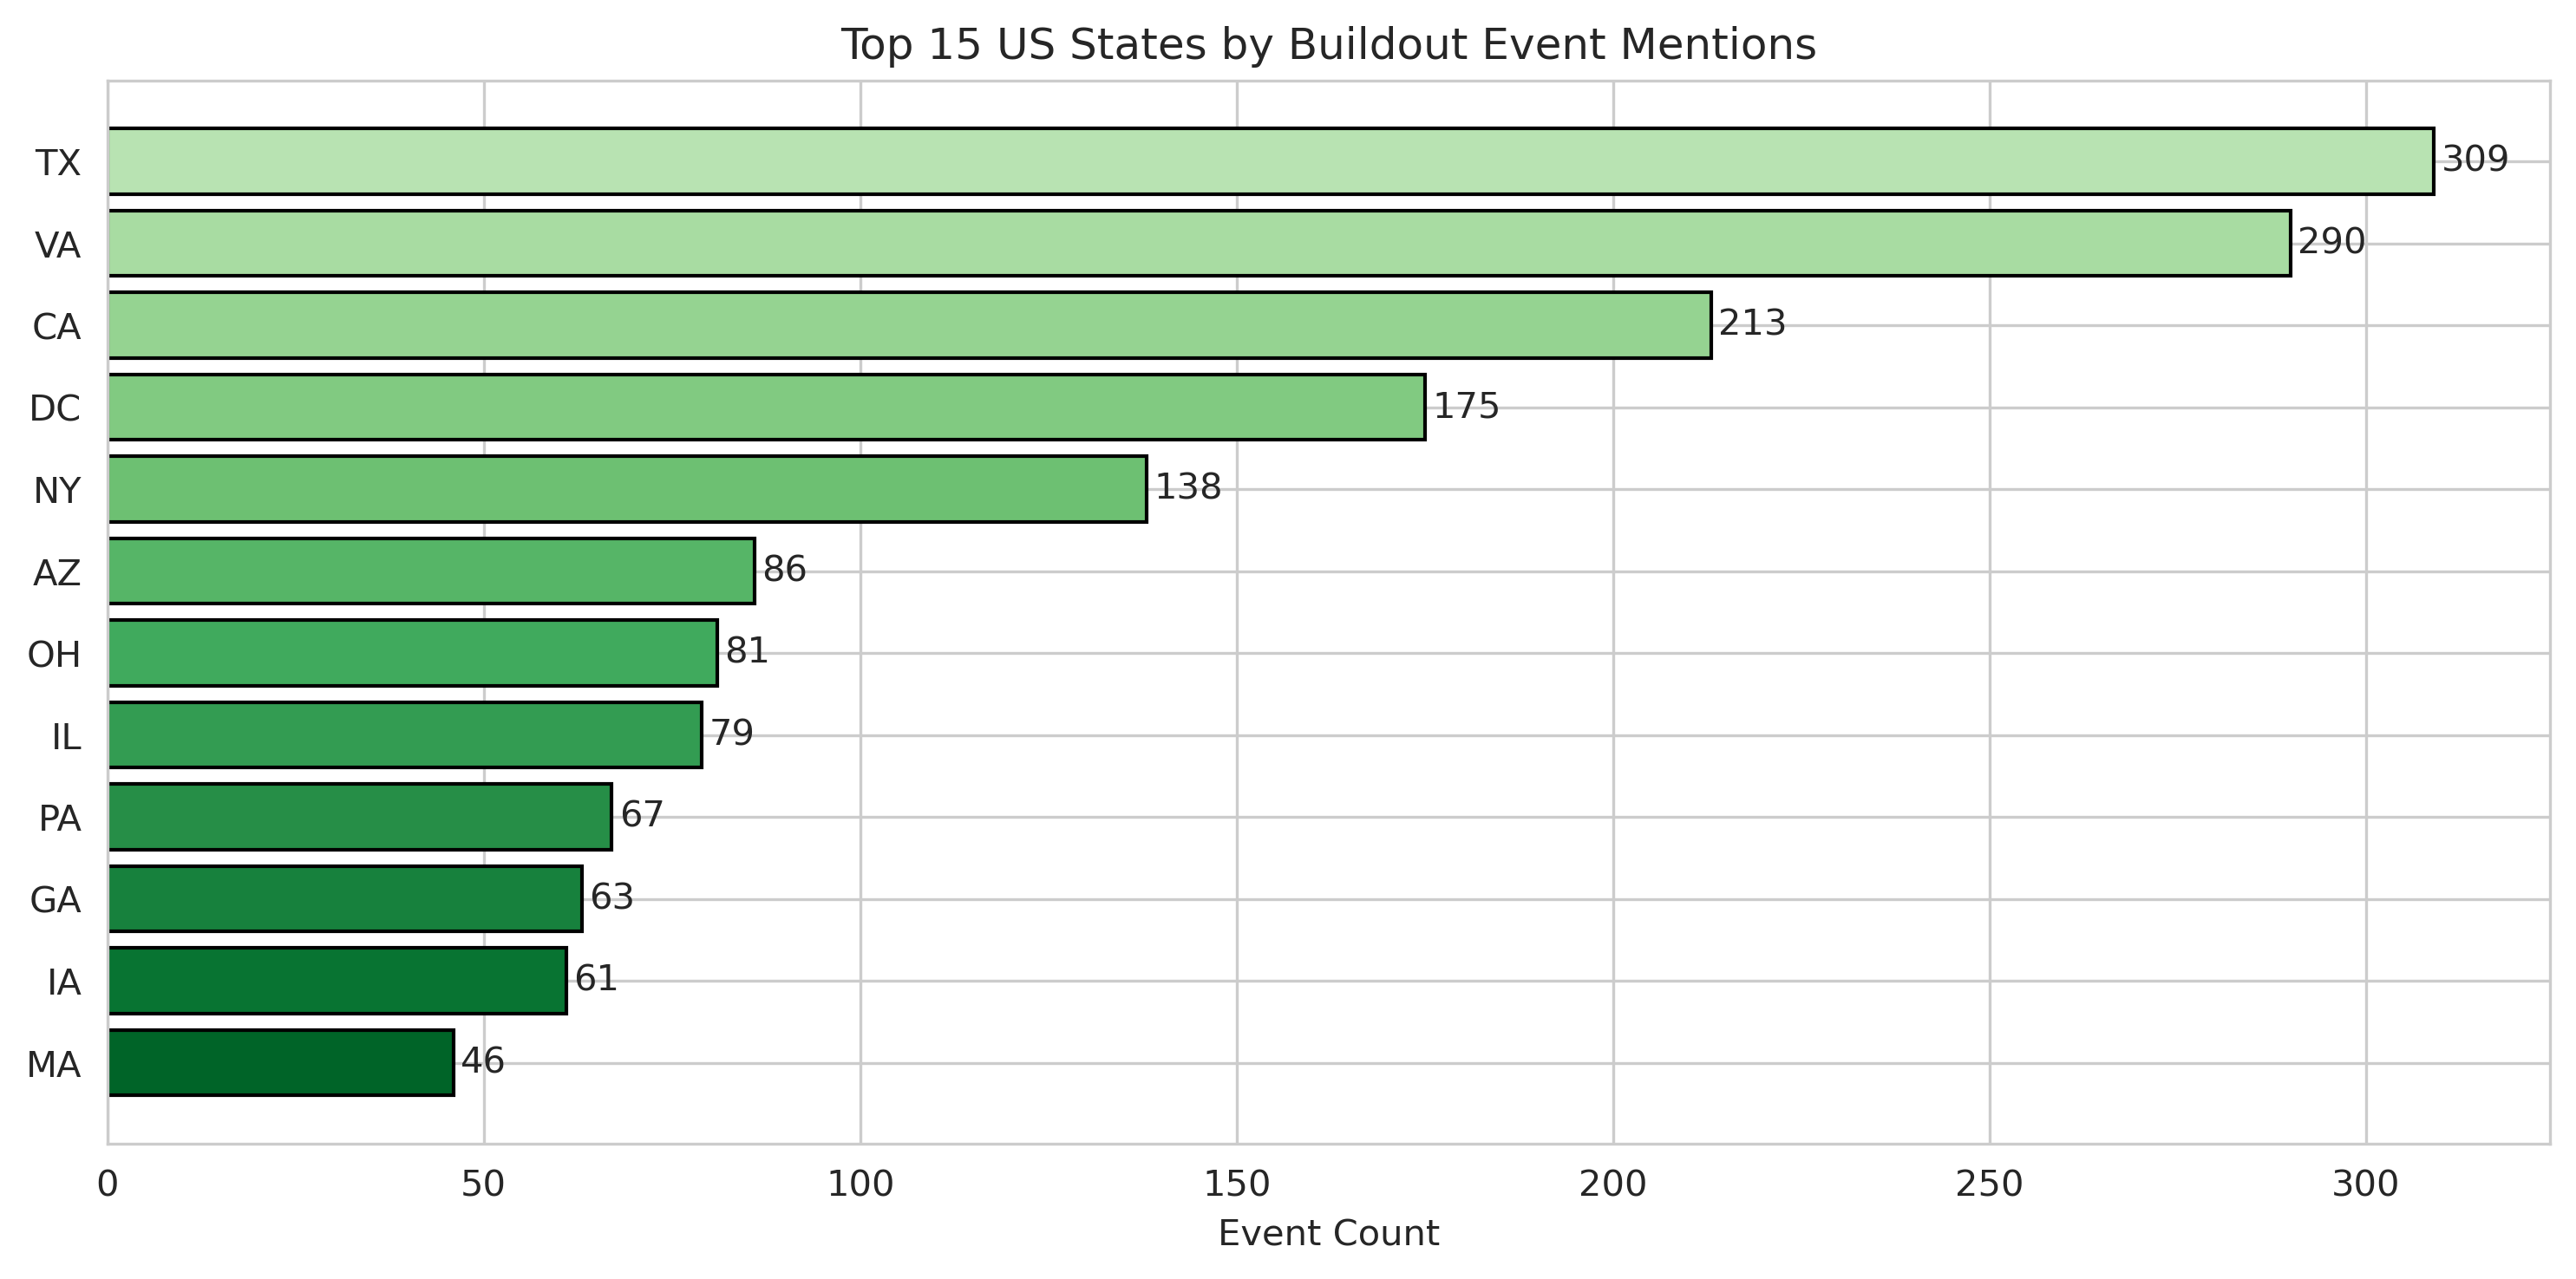
\includegraphics[width=\columnwidth]{../reports/figures/fig6_state_distribution.png}
  \caption{Geographic distribution across U.S. states. Top three: Texas, Virginia, California.}
  \label{fig:state_dist}
\end{figure*}

State-level data is available for 2,246 announcements (42\%). Texas leads with 309 (13.8\%), followed by Virginia (290, 12.9\%), California (213, 9.5\%), and DC (175, 7.8\%). Virginia's prominence reflects Loudoun County's ``Data Center Alley''~\cite{JLARC2024Virginia}. New York has the highest mean MW capacity (4,850~MW), driven by large-scale campus projects.

\subsection{Outcome Classification}

\begin{table*}[t]
\centering
\caption{Distribution of Outcome Labels}
\label{tab:label_dist}
\footnotesize
\begin{tabular}{lrrrr}
\toprule
\textbf{Group} & \textbf{Kept} & \textbf{Failed} & \textbf{Pending} & \textbf{\% Kept} \\
\midrule
\multicolumn{5}{l}{\textit{Overall}} \\
\quad All & 105 & 22 & 5168 & 82.68 \\
\addlinespace
\multicolumn{5}{l}{\textit{By company (selected)}} \\
\quad Microsoft       & 34 & 8 & 1608 & 80.95 \\
\quad Digital Realty  & 20 & 2 & 733  & 90.91 \\
\quad AWS             & 22 & 2 & 688  & 91.67 \\
\quad Google          & 9  & 3 & 686  & 75.00 \\
\quad NVIDIA          & 8  & 1 & 616  & 88.89 \\
\quad Facebook        & 5  & 4 & 229  & 55.56 \\
\addlinespace
\multicolumn{5}{l}{\textit{By confidence}} \\
\quad High   & 39 & 12 & 2110 & 76.47 \\
\quad Medium & 49 & 4  & 1934 & 92.45 \\
\quad Low    & 17 & 6  & 1124 & 73.91 \\
\bottomrule
\end{tabular}
\footnotesize \textit{Note:} 2.0\% completed, 0.4\% failed, 97.6\% pending.
\end{table*}

Only 105 announcements (2.0\%) confirmed completed and 22 (0.4\%) failed. Among 127 with known outcomes, 82.7\% were kept---higher than the 13\% of queue capacity reaching operations~\cite{Rand2025QueuedUp}, likely because press coverage favors successful projects. Facebook/Meta has the lowest keep rate (55.6\%).

\subsection{Sentiment Analysis}

\begin{table*}[t]
\centering
\caption{Characteristics by Outcome}
\label{tab:by_outcome}
\footnotesize
\begin{tabular}{lrrrrrr}
\toprule
\textbf{Characteristic} & \textbf{Kept} & \textbf{Failed} & \textbf{Pending} & \textbf{Diff.} & \textbf{p-value} \\
\midrule
\multicolumn{6}{l}{\textit{MW capacity}} \\
\quad N      & 24   & 5    & 1609 &      & \\
\quad Mean   & 221.42 & 112.80 & 1253.44 & 108.62 & 0.1242 \\
\midrule
\multicolumn{6}{l}{\textit{Tone (v2\_tone)}} \\
\quad N      & 105  & 22   & 5168 &      & \\
\quad Mean   & 1.38 & $-$1.55 & 0.92 & 2.93 & $<$0.001 \\
\midrule
\multicolumn{6}{l}{\textit{Source domain}} \\
\quad datacenterdynamics.com  & 81 & 11 & 3431 & & \\
\quad datacenterknowledge.com & 24 & 11 & 1737 & & \\
\bottomrule
\end{tabular}
\footnotesize \textit{Note:} Welch's $t$-test, Kept vs.\ Failed. Tone difference is highly significant (p $<$ 0.001).
\end{table*}

Completed announcements have mean tone 1.38 (positive), failed $-$1.55 (negative)---a difference of 2.93 (p $<$ 0.001), suggesting linguistic framing contains predictive signal. MW differences are not statistically significant.

\begin{figure*}[t]
  \centering
  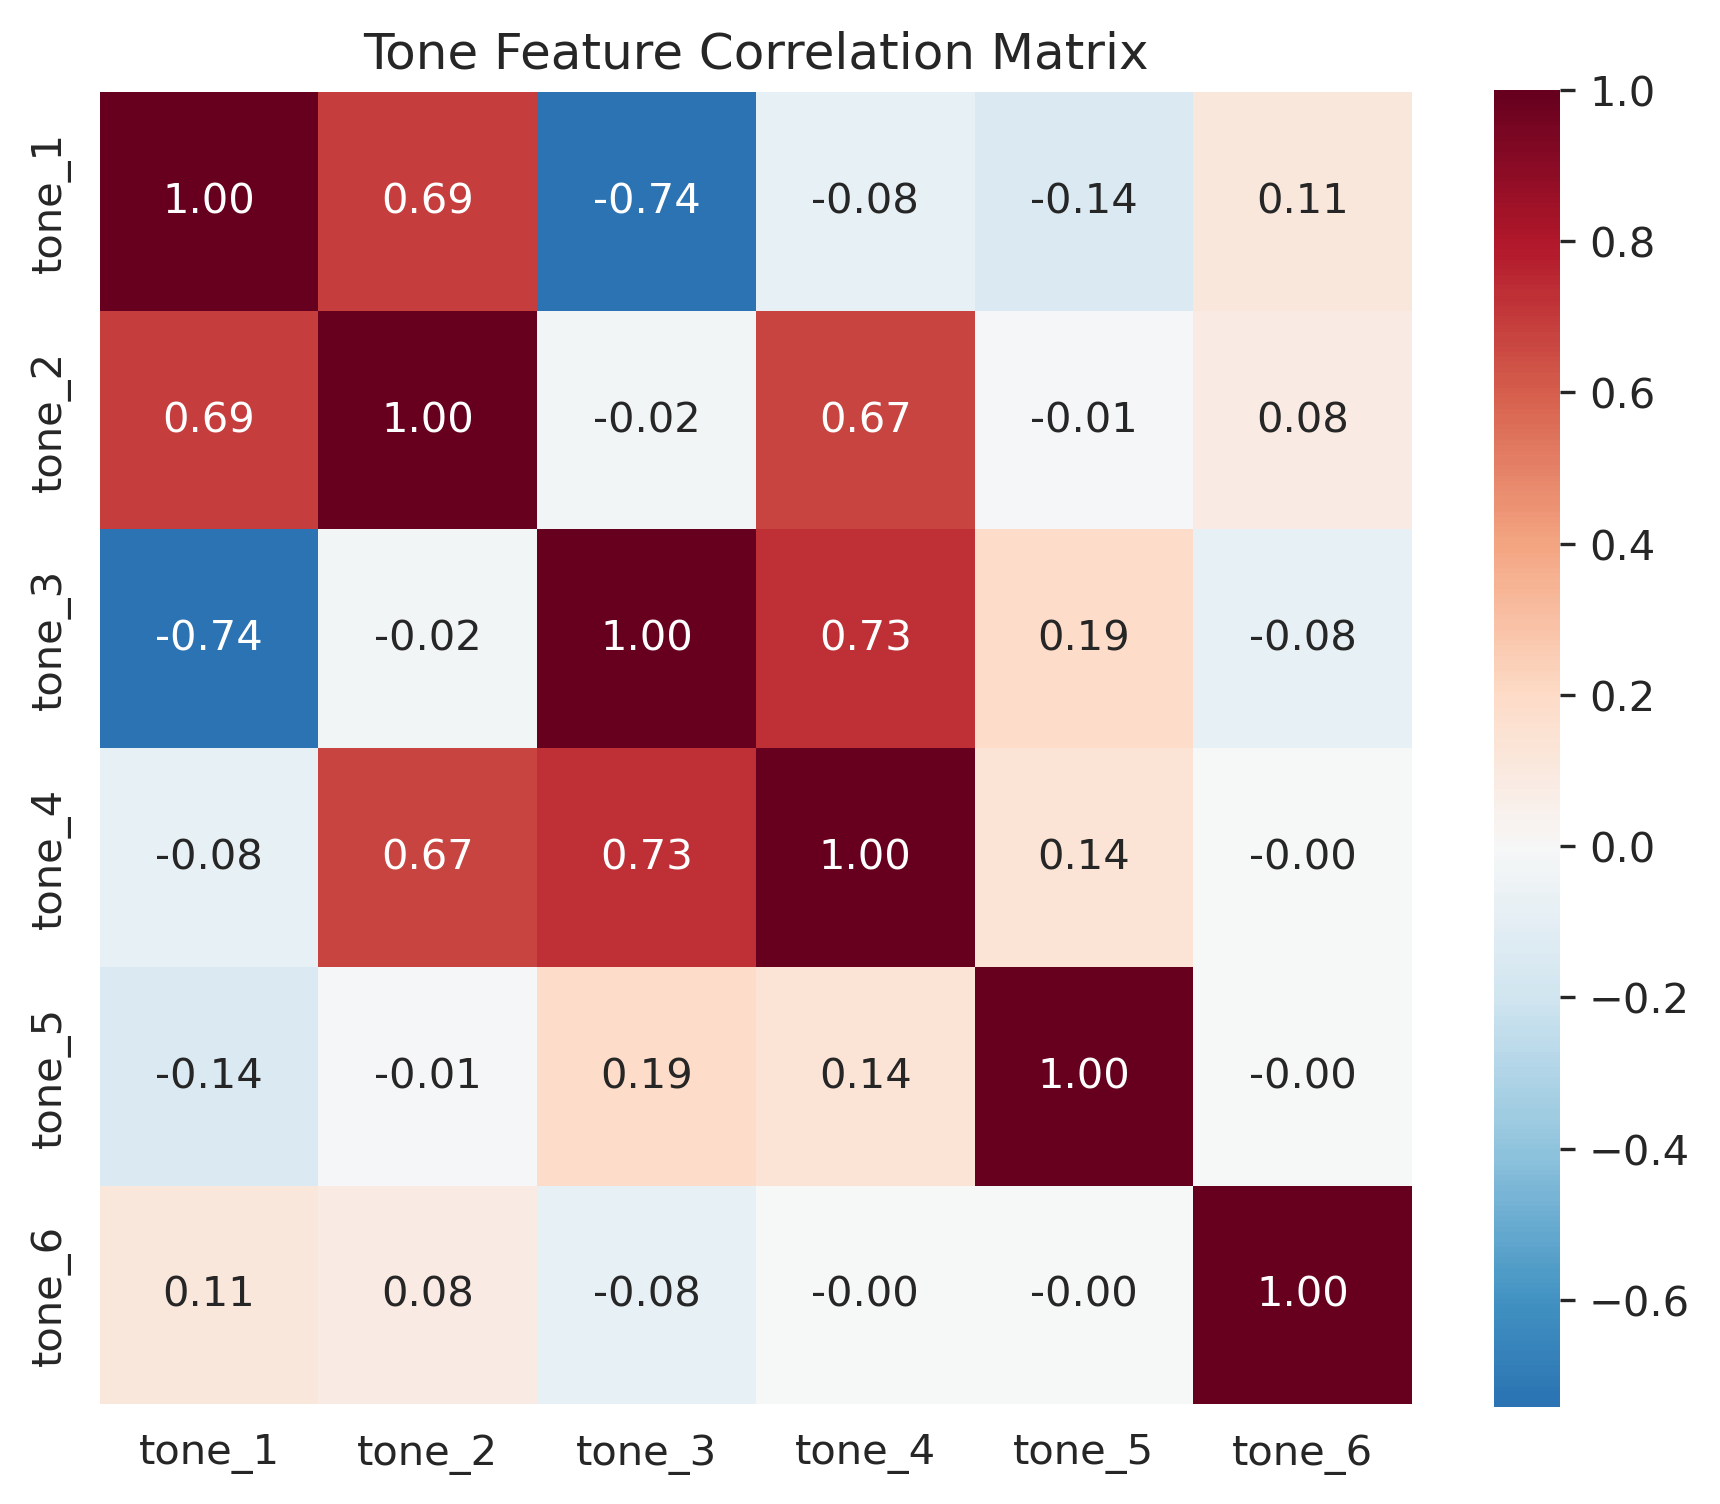
\includegraphics[width=\columnwidth]{../reports/figures/fig8_tone_correlation.png}
  \caption{Announcement tone by outcome. Kept announcements center on positive values; failed cluster in negative territory.}
  \label{fig:tone_dist}
\end{figure*}

\subsection{Event Study Results}

We computed CARs for 1,456 unique events. The $[-1,+1]$ window showed slightly positive but insignificant mean CAR. The $[-5,+5]$ window showed modest positive returns for hyperscaler announcements. The $[-20,+60]$ window revealed substantial cross-sectional variance. Hyperscaler announcements produced more positive CARs than those from smaller REITs, consistent with the investment announcement literature~\cite{MacKinlay1997Event}.

%% ======================================================================
%% 4. DISCUSSION
%% ======================================================================
\section{Discussion}
\label{sec:discussion}

The overwhelming majority of announcements (97.6\%) remain pending, consistent with multi-year lead times: LBNL~\cite{Rand2025QueuedUp} reports median interconnection timelines exceeding four years, and transformer lead times now exceed 160 weeks~\cite{DCKnowlege2026Delays}. Many 2023--2026 announcements may not reach operational status until 2028--2030.

The significant tone-outcome relationship (p $<$ 0.001) is our most actionable finding. Positive tone of kept versus negative tone of failed announcements suggests framing carries predictive signal, consistent with construction ML literature~\cite{Fitzsimmons2022Construction}. This could serve as a leading indicator for investors and grid operators.

\subsection*{Limitations}
First, outcome classification relies on manual verification from industry press, introducing selection bias. The 82.7\% keep rate among labeled outcomes likely overstates the true rate. Second, data is limited to three English-language sources; future work should incorporate permitting records and satellite imagery~\cite{SynMax2026Satellite}. Third, GDELT's single tone score lacks nuance. Fourth, 97.6\% pending means conclusions are based on a small labeled subset. Fifth, the simple market model could benefit from multi-factor approaches~\cite{GoldsmithPinkham2025Financial}.

%% ======================================================================
%% 5. CONCLUSION
%% ======================================================================
\section{Conclusion}
\label{sec:conclusion}

This paper presents the first large-scale empirical analysis of data center buildout announcements. Three principal findings emerge.

First, the landscape is characterized by extreme uncertainty: only 2.0\% confirmed completed, 0.4\% failed, 97.6\% pending---underscoring multi-year lead times and execution risk. Second, announcement tone contains significant predictive signal: kept (mean 1.38) vs.\ failed ($-$1.55) at p $<$ 0.001. Third, market reactions are heterogeneous, with hyperscaler announcements eliciting more positive responses.

For investors, monitoring announcement framing could inform capital allocation. For grid operators, the volume of pending announcements underscores the need for robust planning. For researchers, our dataset provides a foundation for predictive models~\cite{Fitzsimmons2022Construction,Mosca2026AI,Johnston2023Empirical,Rand2025QueuedUp,Zarayeneh2026Multi}. Future work should incorporate permitting records, satellite imagery~\cite{SynMax2026Satellite}, and local opposition tracking~\cite{DataCenterWatch2025Q1}, alongside more sophisticated text analysis and predictive modeling.

\subsection*{Data Availability Statement}
The dataset derived from GDELT is available upon request. GDELT data is public at \url{https://www.gdeltproject.org/data.html}. Code at \url{https://github.com/Aidas-dev/computer-data-analysis-report}.

\subsection*{Ethics Declaration}
This research uses publicly available news and stock price data. No human subjects were involved.

\subsection*{CRediT Author Contribution Statement}
\textbf{Aidas:} Conceptualization, Methodology, Software, Validation, Formal analysis, Investigation, Data Curation, Writing -- Original Draft, Writing -- Review \& Editing, Visualization, Supervision, Project administration.

\subsection*{Conflict of Interest Statement}
The author declares no competing financial or non-financial interests.

\subsection*{Funding Acknowledgment}
This research received no specific grant from any funding agency.

\subsection*{AI Disclosure Statement}
Portions of the data processing pipeline and literature synthesis were assisted by large language models. All analyses were reviewed and validated by the author.

\subsection*{Acknowledgments}
The author thanks the GDELT Project for making its Global Knowledge Graph publicly available.

%% Bibliography
\bibliographystyle{elsarticle-num}
\bibliography{references}

\end{document}
